\chapter{\uppercase{Introduction}}


%\begin{spacing}{1.5}\section*{\LARGE{\mdseries{Thesis Outline}}}

 

  Arabic is the fifth most widely spoken language\footnote{\textit{according to the 20th edition of Ethnologue, 2017}}. It is written from right to left. Its
alphabet consists of 28 primary letters, and there are 8 more derived letters
from the basic ones, so the total count of Arabic characters is 36 characters.
The writing system is cursive; hence, most letters join to the letter that comes
after them, a few letters remain disjoint.

\section{Arabic Poetry } %%
%% Introduction; the circumstances before alarud
Arabic poetry(\textarabic{الشعر العربى}) is the earliest form of Arabic literature. It dates back to the Sixth century. Poets have written poems without knowing exactly what rules which make a collection of words a poem. People recognize poetry by nature, but only talented ones can write poems. This was the case until \textit{Al-Farahidi} (718 – 786 CE) has analyzed the
Arabic poetry, then he came up with that the succession of consonants and vowels
produce patterns or \textit{meters}, which make the music of poetry.  He has
counted them fifteen meters.  After that, a student of \textit{Al-Farahidi} has
added one more meter to make them sixteen. Arabs call meters \textarabic{بحور}
which means ``\textit{seas}''. The study of Arabic Poems classification is named \textbf{Al-Arud (\textarabic{العَروض})}. It takes too much time for anyone to be an expert in this field. 
\section{Deep Learning}

Deep Learning also named Deep Neural Network is part of Machine Learning algorithms. Deep Learning is trying to simulate the human brain into Neural dependency.  Using Deep Learning, we can achieve better learning results from the data. Deep Neural Network needs a huge amount of data to achieve the expected learning curve and results. It also needs a massive amount of computation to build the networks which are based on an artificial neural network. We used the Recurrent Neural Network (RNN) to work on the Arabic Text which shown its ability to achieve outstanding performance over the text problem data. We also used LSTM to solve the long dependency issue in RNN. We will go deep into the Background section (add deep learning section reference).

\section{Thesis Objectives}
In this study, we work to classify the poem and utilize the latest technologies check the class of poem. We also worked to achieve near human expert results which make our work is a breakthrough in the field concerning the results compared to the current achieved results. Figure \ref{fig:thesis_cycle} shows the steps.,
\begin{figure}[h!]
  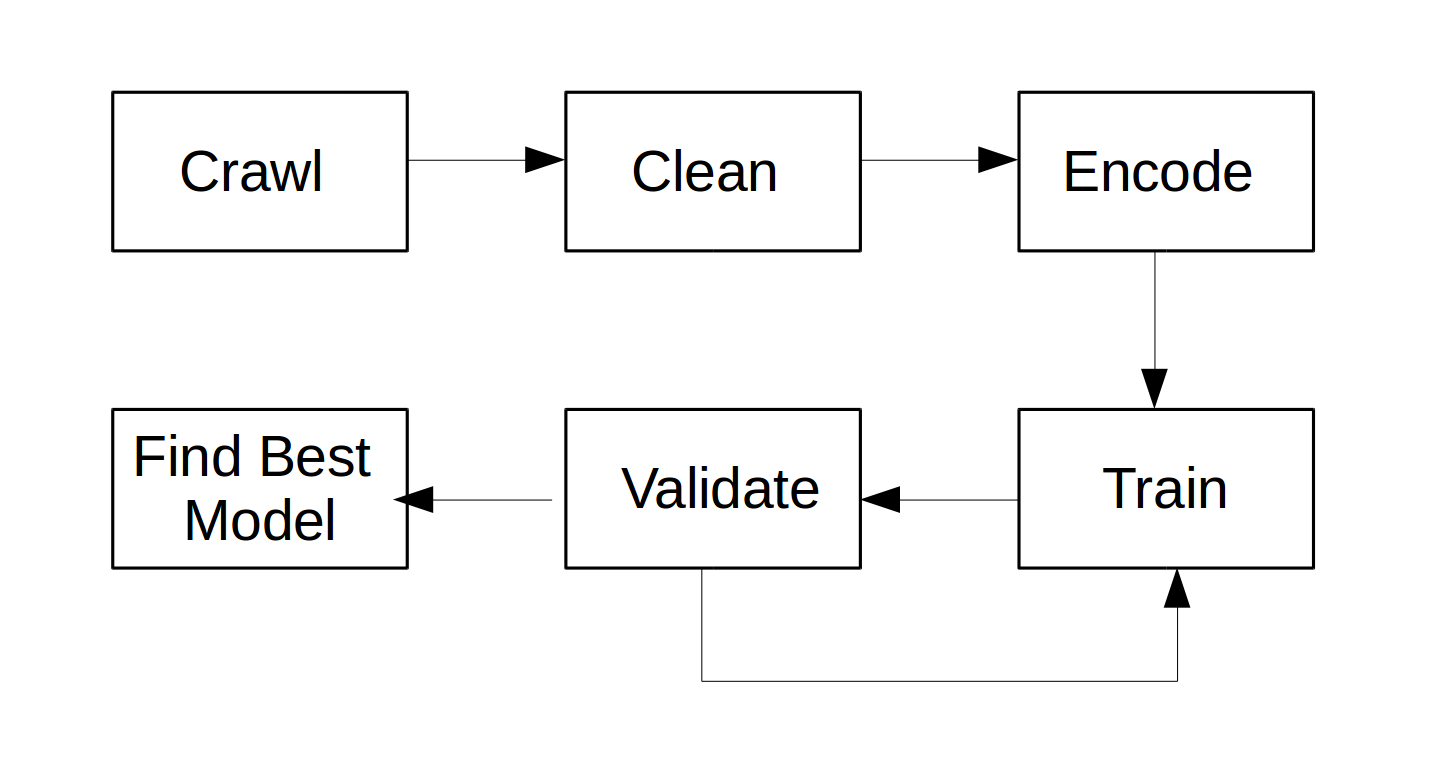
\includegraphics[width=\linewidth,height=6cm]{./Figures/Ch_1_Intro/Master_Cycle.png}
  \caption{Thesis Working Steps.}
  \label{fig:thesis_cycle}
\end{figure}

\begin{itemize}
\item Crawling the data from the available sources with labeling.
\item Clean and transform the data.
\item Encode the data into a way to be input to the model to work on it. We used many encoding methods and compared each of them.
\item Train the RNN model into the cleaned data.
\item Validate and test the model.
\item Enhance the model.

\end{itemize}








%\begin{figure}
%	
%	

\begin{tikzpicture}[scale=0.9]
\begin{axis}[
    symbolic x coords={Taweel,
   Kamel,
   Baseet,
   Khafeef,
   Wafeer,
   Rigz,
   Raml,
   Motakarib,
   Sar'e,
   Monsafeh,
   Mogtath,
   Madeed,
   Hazg,
   Motadarik,
   Moktadib,
   Modar'e
    },
    xtick=data,
    % the following x label positioning does work here.
    every axis y label/.style= {at={( 0.1, 1.1)}, anchor=north},
    %ylabel style={font=\footnotesize},
    xticklabel style = {font=\footnotesize},
    ylabel={Class size},
    x=0.4cm,
    x tick label style={rotate=60, anchor=east}, 
    % Y ticks configurations
    y tick label style={/pgf/number format/.cd,%
      scaled y ticks = false,
      set thousands separator={,},
      fixed},]
    \addplot[ybar,fill=myBlue] coordinates {
        (Taweel, 416428)
        (Kamel,  370116)
        (Baseet, 244583)
        (Khafeef,     157880)
        (Wafeer,     143148)
        (Rigz,     119286)
        (Raml,     79560)
        (Motakarib,     63613)
        (Sar'e,     59370)
        (Monsafeh,     28768)
        (Mogtath,     18062)
        (Madeed,     7808)
        (Hazg,     7468)
        (Motadarik,     5144)
        (Moktadib,     799 )
        (Modar'e,     288 )
    };
\end{axis}
\end{tikzpicture}

%	
%	\caption{Meter names are on the $x$-axis, size  is on the $y$-axis.}
%	\label{data_size}
%\end{figure}



